\section{Tracking Techniques}
\label{sec:tracking-techniques}

%%
Our literature review described in \autoref{sec:lit-review} identifies 58 papers that provide a foundational understanding of specific web tracking techniques, complemented by 108 measurement studies that characterize their real-world aspects.
%
The systematization of this literature as per the approach explained in~\autoref{sec:systematization} yields 24 distinct tracking techniques.
%
\autoref{tab:technique-papers} maps these 58 tracking technique papers against the techniques they study.


%%
Fundamentally, each tracking technique relies on artifacts tied either to the user, their device, or their browsing activity to achieve tracking goals listed in \autoref{tab:systematization-criteria}.
%
To this end, across the above described literature, we systematize the artifacts that trackers were observed to rely on in different papers into eight categories (\autoref{tab:artifact-taxonomy}). 
%
A paper-level overview of the tracked artifacts and the capabilities defined in \autoref{sec:threat-model} (i.e., \symInclusion~Inclusion, \symExecution~Execution, \symObservation~Observation, \symStorage~Storage, \symSharing~Sharing) that are exercised by the trackers over each artifact category is represented in \autoref{tab:paper-artifacts} (\refappendix{?}). 
%
\autoref{tab:artifact-capability-matrix} systematizes these tracker capabilities across artifacts for each tracking technique. 


%%
Overall, we can observe trackers to exercise \symSharing~Sharing and \symInclusion~Inclusion capabilities with nearly every technique, since a tracker must always be included directly or indirectly within a webpage and eventually exfiltrate what it collects to be able to track. 
%
On the other hand, \symStorage~Storage is essentially exclusive to the techniques we classify as stateful that require it to maintain state across contexts, while \symObservation~Observation is concentrated with the passive or out-of-band techniques (e.g., network- and hardware-oriented techniques).


%%
\begin{table*}[t]
\centering
\scriptsize
\setlength{\tabcolsep}{1pt}
\renewcommand{\arraystretch}{1}
\caption{Tracker capabilities most commonly exercised over each artifact (rows) for each tracking technique (columns). \protect\symInclusion~Inclusion, \protect\symExecution~Execution, \protect\symStorage~Storage, \protect\symSharing~Sharing, \protect\symObservation~Observation.}
\label{tab:artifact-capability-matrix}
\begin{tabular}{%
|>{\raggedright\arraybackslash}m{3.0cm}|>{\centering\arraybackslash}m{0.63cm}|>{\centering\arraybackslash}m{0.63cm}|>{\centering\arraybackslash}m{0.63cm}|>{\centering\arraybackslash}m{0.63cm}|>{\centering\arraybackslash}m{0.63cm}|>{\centering\arraybackslash}m{0.63cm}|>{\centering\arraybackslash}m{0.63cm}|>{\centering\arraybackslash}m{0.63cm}|>{\centering\arraybackslash}m{0.63cm}|>{\centering\arraybackslash}m{0.63cm}|>{\centering\arraybackslash}m{0.63cm}|>{\centering\arraybackslash}m{0.63cm}|>{\centering\arraybackslash}m{0.63cm}|>{\centering\arraybackslash}m{0.63cm}|>{\centering\arraybackslash}m{0.63cm}|>{\centering\arraybackslash}m{0.63cm}|>{\centering\arraybackslash}m{0.63cm}|>{\centering\arraybackslash}m{0.63cm}|>{\centering\arraybackslash}m{0.63cm}|>{\centering\arraybackslash}m{0.63cm}|%
}
\toprule
\multicolumn{1}{|>{\centering\arraybackslash}b{3.0cm}|}{\shortstack[c]{\textbf{Tracked}\\\textbf{Artifacts}}} & \multicolumn{1}{>{\centering\arraybackslash}b{0.63cm}|}{\rot{Third-party Cookie Tracking}} & \multicolumn{1}{>{\centering\arraybackslash}b{0.63cm}|}{\rot{Cookie Respawning}} & \multicolumn{1}{>{\centering\arraybackslash}b{0.63cm}|}{\rot{Cookie Syncing}} & \multicolumn{1}{>{\centering\arraybackslash}b{0.63cm}|}{\rot{First-party Cookie Tracking}} & \multicolumn{1}{>{\centering\arraybackslash}b{0.63cm}|}{\rot{Tracking Pixels/Tags}} & \multicolumn{1}{>{\centering\arraybackslash}b{0.63cm}|}{\rot{CNAME Tracking}} & \multicolumn{1}{>{\centering\arraybackslash}b{0.63cm}|}{\rot{Link Decorations}} & \multicolumn{1}{>{\centering\arraybackslash}b{0.63cm}|}{\rot{Bounce Tracking}} & \multicolumn{1}{>{\centering\arraybackslash}b{0.63cm}|}{\rot{Authentication-based Tracking}} & \multicolumn{1}{>{\centering\arraybackslash}b{0.63cm}|}{\rot{Cross-context Tracking}} & \multicolumn{1}{>{\centering\arraybackslash}b{0.63cm}|}{\rot{Javascript-based Tracking}} & \multicolumn{1}{>{\centering\arraybackslash}b{0.63cm}|}{\rot{Browser Fingerprinting}} & \multicolumn{1}{>{\centering\arraybackslash}b{0.63cm}|}{\rot{Extension Fingerprinting}} & \multicolumn{1}{>{\centering\arraybackslash}b{0.63cm}|}{\rot{Device Fingerprinting}} & \multicolumn{1}{>{\centering\arraybackslash}b{0.63cm}|}{\rot{Passive Fingerprinting}} & \multicolumn{1}{>{\centering\arraybackslash}b{0.63cm}|}{\rot{Kernel-based Side-channels}} & \multicolumn{1}{>{\centering\arraybackslash}b{0.63cm}|}{\rot{Network-based Side-channels}} & \multicolumn{1}{>{\centering\arraybackslash}b{0.63cm}|}{\rot{Timing-based Side-channels}} & \multicolumn{1}{>{\centering\arraybackslash}b{0.63cm}|}{\rot{Storage-based Side-channels}} & \multicolumn{1}{>{\centering\arraybackslash}b{0.63cm}|}{\rot{Behavioral Tracking}} \\
\midrule
\rh Browser Storage and Cache & \cellsym{\symStorage} & \cellsym{\symStorage} & \cellsym{\symStorage} & \cellsym{\symStorage} & \cellsym{\symStorage} & \cellsym{\symStorage} & \cellsym{\symStorage} & \cellsym{\symStorage} & \cellsym{\symStorage} & \cellsym{\symStorage} & \cellsym{\symStorage} & \ec & \ec & \ec & \ec & \ec & \ec & \ec & \cellsym{\symStorage} & \ec \\
\hline
\rh JS-Accessible Browser APIs & \cellsym{\symExecution} & \cellsym{\symExecution} & \cellsym{\symExecution} & \cellsym{\symExecution} & \cellsym{\symExecution} & \ec & \ec & \cellsym{\symExecution} & \ec & \cellsym{\symExecution} & \cellsym{\symExecution} & \cellsym{\symExecution} & \cellsym{\symExecution} & \cellsym{\symExecution} & \ec & \cellsym{\symExecution} & \ec & \cellsym{\symExecution} & \cellsym{\symExecution} & \cellsym{\symExecution} \\
\hline
\rh Webpage Artifacts & \cellsym{\symInclusion} & \cellsym{\symInclusion} & \cellsym{\symInclusion} & \cellsym{\symInclusion} & \cellsym{\symInclusion\,\symExecution} & \cellsym{\symInclusion} & \cellsym{\symInclusion} & \cellsym{\symInclusion} & \cellsym{\symInclusion} & \cellsym{\symInclusion} & \cellsym{\symInclusion\,\symExecution} & \cellsym{\symInclusion\,\symExecution} & \cellsym{\symInclusion\,\symExecution} & \cellsym{\symInclusion\,\symExecution} & \cellsym{\symInclusion} & \cellsym{\symInclusion} & \ec & \cellsym{\symInclusion} & \cellsym{\symInclusion} & \cellsym{\symInclusion\,\symExecution} \\
\hline
\rh Hardware Artifacts & \ec & \ec & \ec & \ec & \ec & \ec & \ec & \ec & \ec & \cellsym{\symExecution\,\symObservation} & \ec & \ec & \ec & \cellsym{\symExecution\,\symObservation} & \ec & \cellsym{\symExecution\,\symObservation} & \ec & \cellsym{\symExecution\,\symObservation} & \ec & \ec \\
\hline
\rh Network Protocol Artifacts & \ec & \ec & \ec & \ec & \ec & \cellsym{\symSharing} & \ec & \ec & \ec & \ec & \ec & \ec & \ec & \cellsym{\symObservation} & \cellsym{\symObservation} & \cellsym{\symObservation} & \cellsym{\symObservation} & \ec & \ec & \ec \\
\hline
\rh HTTP Traffic Artifacts & \cellsym{\symSharing} & \cellsym{\symSharing} & \cellsym{\symSharing} & \cellsym{\symSharing} & \cellsym{\symSharing} & \cellsym{\symSharing} & \cellsym{\symSharing} & \cellsym{\symSharing} & \cellsym{\symSharing} & \cellsym{\symSharing} & \cellsym{\symSharing} & \cellsym{\symSharing} & \cellsym{\symSharing} & \cellsym{\symSharing} & \cellsym{\symSharing} & \cellsym{\symSharing} & \cellsym{\symObservation} & \cellsym{\symSharing} & \cellsym{\symSharing} & \cellsym{\symSharing} \\
\hline
\rh Navigational Artifacts & \ec & \ec & \cellsym{\symSharing} & \ec & \cellsym{\symSharing} & \ec & \cellsym{\symSharing} & \cellsym{\symSharing} & \cellsym{\symSharing} & \ec & \ec & \ec & \ec & \ec & \ec & \ec & \ec & \ec & \ec & \ec \\
\hline
\rh Identifiers & \cellsym{\symStorage\,\symSharing} & \cellsym{\symStorage\,\symSharing} & \cellsym{\symStorage\,\symSharing} & \cellsym{\symStorage\,\symSharing} & \cellsym{\symStorage\,\symSharing} & \cellsym{\symStorage\,\symSharing} & \cellsym{\symSharing} & \cellsym{\symStorage\,\symSharing} & \cellsym{\symStorage\,\symSharing} & \cellsym{\symStorage\,\symSharing} & \cellsym{\symStorage\,\symSharing} & \cellsym{\symSharing} & \cellsym{\symSharing} & \cellsym{\symSharing} & \ec & \ec & \ec & \ec & \ec & \ec \\
\bottomrule
\end{tabular}
% \vspace{-2mm}
\end{table*}


%%
We organize the remainder of this section by tracked state (\autoref{tab:systematization-criteria}), discussing the evolution of each technique under three categories: \textit{stateful} tracking (\autoref{sec:stateful-tracking}), \textit{stateless} tracking (\autoref{sec:stateless-tracking}), and \textit{mixed} tracking (\autoref{sec:mixed-techniques}).
%
Within each, we highlight research gaps and identify open problems that will shape future research directions for each technique.
%
% \autoref{fig:evolution-techniques} plots the evolutionary milestones underlying our systematization across tracking techniques. 


\begin{comment}
\begin{figure*}
    \centering
    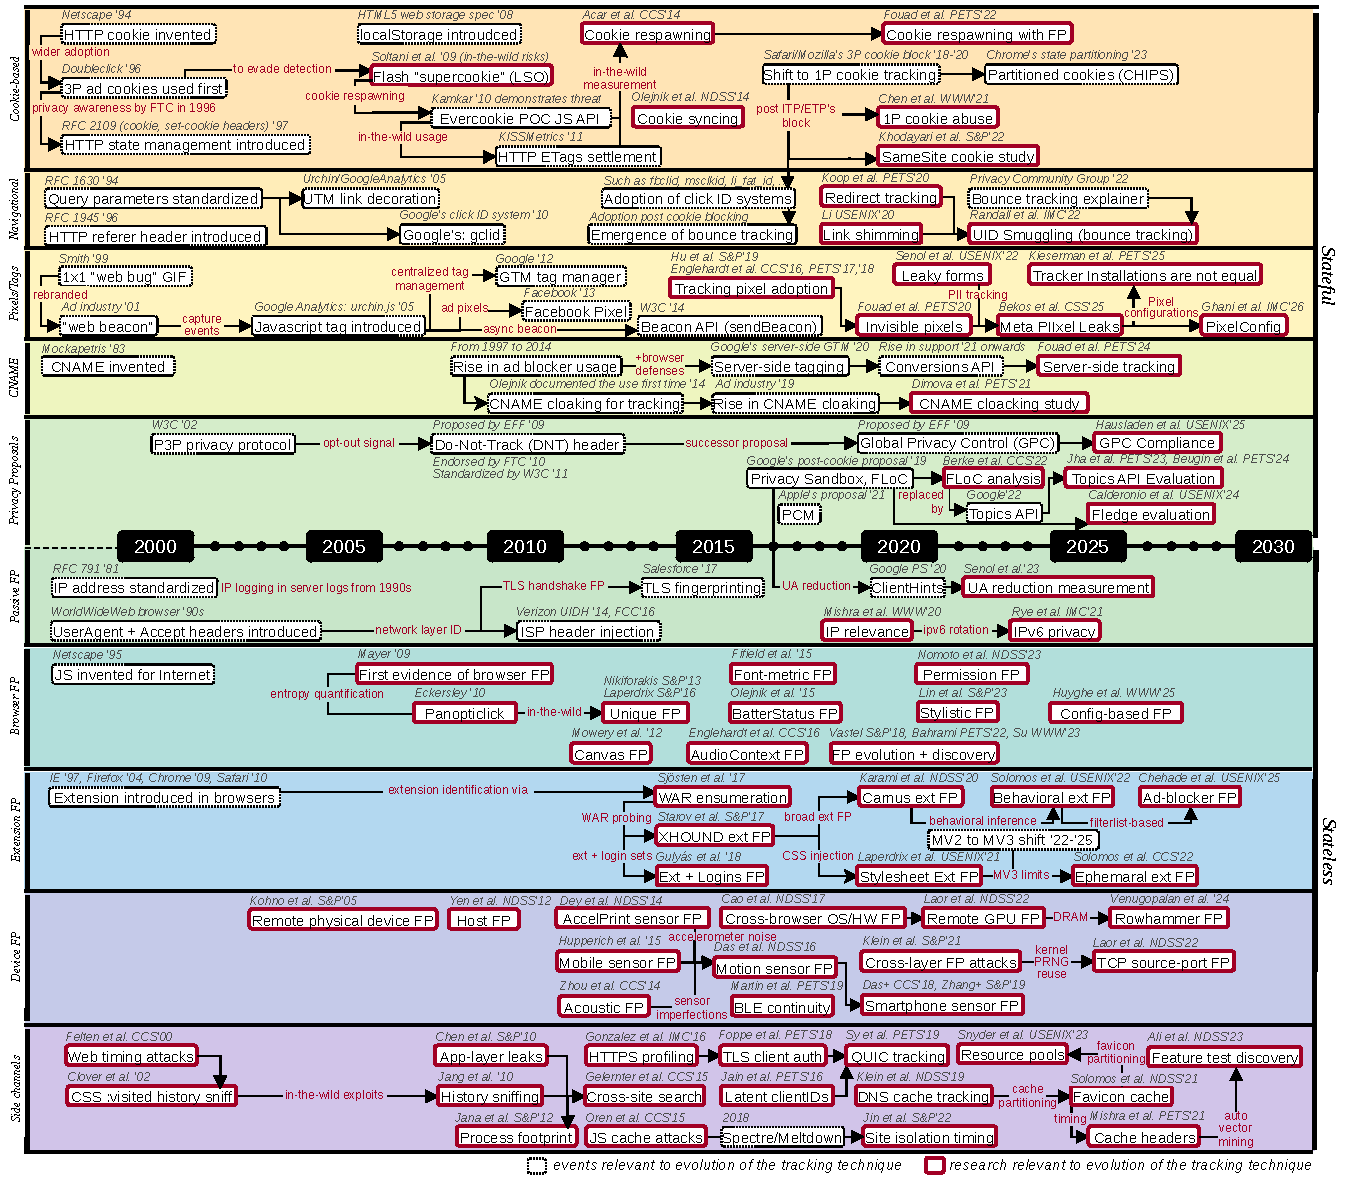
\includegraphics[width=1\linewidth]{long-version/evolution-tracking-techniques.pdf}
    \caption{Evolution of research on stateful and stateless web tracking techniques.}
    \label{fig:evolution-techniques}
\end{figure*}
\end{comment}



%%
\subsection{Stateful Tracking}
\label{sec:stateful-tracking}
%%
The most straightforward approach to tracking a user involves storing a unique identifier in their browser and retrieving it or modifying it as they browse different websites, through techniques that can be categorized as \textit{stateful tracking}.
%
Browsers provide a number of interfaces (e.g., cookies) that are designed to associate \textit{state} to the user's visit, and others that store information as a side effect of some other functionality (e.g., E-Tags, HSTS upgrades), which trackers sometimes abuse to encode a unique identifier~\cite{englehardtAutomatedDiscoveryPrivacy2018,ashkansoltaniFlashCookiesPrivacy2011,solomosTalesFaviconsCaches2021}.


%%
Historically, stateful tracking relied primarily on third-party storage, allowing the same identifier to be read across unrelated websites.
%
However, modern browsers now either block~\cite{TrackingPreventionWebKit2020} or partition third-party access to stateful APIs by origin~\cite{mdnThirdpartyCookiesPrivacy2024}, preventing trackers from storing and retrieving identifiers across sites.
%
As a result, tracking has increasingly shifted into the first-party context, where third-party services store site-specific identifiers and subsequently link them across websites using additional reconciliation mechanisms (e.g., logged-in account information).
%
Accordingly, this section systematizes stateful tracking techniques in both third- and first-party tracking contexts.












%%
\subsubsection{Cookie-based Tracking}
\label{sec:stateful-techniques-cookies}

%%
Cookies---first specified by Lou Montulli at Netscape in the 1990s---allow maintaining a state when the browser communicates with a web server via HTTP, a stateless protocol~\cite{kristolHTTPCookiesStandards2001}.
%
For example, a website can store a user's authentication token in the browser via a cookie, which is then shared with the web server with each request that the user's browser makes, allowing the website to verify the user's authentication status.
%
Browsers mediate which resources and domains are able to access specific cookies~\cite{beugin2024WebAlmanac2024,singhIncoherenciesWebBrowser2010,mdnSameoriginPolicySecurity2024}.


%%
Cookie-based tracking primarily relies on browser storage \symStorage\ (specifically cookie jar) to maintain state. 
%
First- or third-party domains included \symInclusion\ on a webpage can set and receive cookies through \texttt{cookie} and \texttt{set-cookie} headers in network requests and responses respectively (i.e., \symSharing\ over HTTP traffic artifacts) or via the \texttt{document.cookie} or CookieStore JavaScript API (i.e., \symExecution\ using JS APIs).
%
Cookies set in a first-party context on a website are called first-party cookies, allowing a user to be re-identified to the website that they visit.
%
Similarly, cookies set in a third-party context are classified as third-party cookies and they allow cross-site tracking.


%%
Cookies were adopted for cross-site advertising and tracking almost immediately after their introduction, prompting early privacy concerns~\cite{montulliHTTPStateManagement1997,kristolHTTPCookiesStandards2001,SenatorRaisesPrivacy2001}.
%
Despite these concerns, cookie-based tracking remained dominant for nearly two decades: large-scale measurement studies have confirmed these concerns, showing that tracking had become both widespread and concentrated among a small set of dominant third parties, while the number of trackers per page increased steadily over time~\cite{krishnamurthyPrivacyDiffusionWeb2009,lernerInternetJonesRaiders2016,englehardtOnlineTracking1millionsite2016,karajWhoTracksMeShedding2019,yuTrackingTrackers2016}.
%
As Safari and Firefox began blocking third-party cookies by default between 2018 and 2020 (\autoref{sec:stateful-defenses}), tracking largely shifted into the first-party context instead. 
%
Today, nearly 90\% of websites set first-party tracking cookies, 96\% of which are in fact set by third-party scripts running in a first-party context, and browsing with third-party cookies disabled remains largely indistinguishable from the pre-blocking web~\cite{munirCookieGraphUnderstandingDetecting2023,vekaria2024WebAlmanac2024,linBrowsingThirdPartyCookies2024}.
%
Despite this transition, sites continue to opt out of browser protections such as \texttt{SameSite=Lax} and instead rely on \texttt{SameSite=None} cookies, letting first- and third-party cookies remain intertwined in practice~\cite{khodayariStateSameSiteStudying2022}.
%
Moreover, trackers continue exploiting browser- and protocol-level edge cases to retain stateful tracking capabilities~\cite{khodayariStateSameSiteStudying2022,bashirHowTrackingCompanies2018}.


%%
\subsubsection{Cookie Respawning}
\label{sec:stateful-techniques-cookie-respawning}
%%
Once a user clears their cookies, a tracker that has stashed the same identifier somewhere else in the browser can rewrite it back into the cookie jar, ``respawning'' or reconstructing the identifier and creating a so-called ``supercookie'' or ``evercookie''~\cite{ayensonFlashCookiesPrivacy2011,soltaniFlashCookiesPrivacy2009,acarWebNeverForgets2014} as described in \autoref{sec:stateful-defenses-??}.
%
Respawning was first demonstrated at scale using Flash Local Shared Objects and other legacy plugin storage~\cite{acarWebNeverForgets2014,englehardtOnlineTracking1millionsite2016}, and later shown to also draw on browser fingerprints themselves---a 2022 study measured a lower bound on fingerprint-based respawning by detecting it on 1,150 of the top 30K sites~\cite{fouadMyCookiePhoenix2022}.
%
More recently, respawning has expanded beyond the browser, leveraging cross-context state shared with native applications to recover identifiers~\cite{wessels2025hytrack}.
%
% The technique's most recent evolution moves respawning outside the browser altogether: HyTrack shows that Android's Custom Tabs and WebView components, which are designed to let a native app and the system browser share cookies for a seamless login experience, let a tracker resurrect a supercookie-like identifier across app reinstalls, browser switches, and even device backups~\cite{wessels2025hytrack}---a persistence guarantee no purely in-browser respawning technique has ever achieved.
%
We discuss this in detail under cross-context tracking techniques in \autoref{sec:cross-context-techniques}.


%%
\subsubsection{Cookie Syncing}
\label{sec:stateful-techniques-cookie-syncing}
%%
Third-parties included on only a few websites are able to track users only across that limited set of sites~\cite{acarWebNeverForgets2014}.
%
Moreover, under the SOP restriction, a third-party on a webpage cannot share its cookies with another third-party domain by directly initiating a request to it.
%
To overcome these constraints and exchange information collected about the user on different websites, third-party companies rely on cookie syncing or cookie matching~\cite{acarWebNeverForgets2014}---first described by Olejnik et al.~\cite{olejnikSellingPrivacyAuction2014}. % and also named as ``referred tracking'' by Roesner et al.~\cite{roesnerDetectingDefendingThirdparty2012}.
%
This mechanism relies on synchronizing user identifiers known to two different third parties that are typically stored in third-party cookies and most commonly shared via URL parameters exchanged during a redirect between the two trackers. % (see \autoref{subfig:cookie-syncing})
%
Earlier works formalized cookie syncing detection approach~\cite{acarWebNeverForgets2014,englehardtOnlineTracking1millionsite2016,bashirTracingInformationFlows2016} and has since been refined~\cite{papadopoulosCookieSynchronizationEverything2019} and scaled into automated, graph- and ML-based pipelines that trace identifier flows across the wider advertising ecosystem~\cite{papadopoulosCookieSynchronizationEverything2019, iqbalKhaleesiBreakerAdvertising2022}.
%
Moreover, cookie syncing is not confined to the third-party context as identifiers stored in first-party cookies are just as often synced across trackers~\cite{sanchez-rolaJourneyCenterCookie2021}. 
%
Notably, first-party cookies set by Google and Facebook have been observed to be shared with hundreds of other third-party domains~\cite{munirCookieGraphUnderstandingDetecting2023,bahramiCOOKIEGUARDCharacterizingIsolating2024}.



%%
\subsubsection{Tracking Pixels/Tags}
\label{sec:stateful-techniques-tags}

%%
Traditionally, tracking pixels (or invisible pixels) used to be 1x1 image elements embedded \symInclusion\ on a webpage that pointed to some tracking endpoint~\cite{Narayanan2017WebtapSpringer,englehardtOnlineTracking1millionsite2016}.
%
When a user visits a webpage embedding a 1x1 pixel, user data is shared \symSharing\ with the tracker over HTTP traffic artifacts, allowing user tracking on the same site as well as cross-site.
%
Image-based tracking pixels have been primarily used for analytics, ad (re)targeting, and conversion tracking, 
%
Their prevalence and privacy risks have been measured extensively over time~\cite{englehardtOnlineTracking1millionsite2016}, from early archaeological studies of the tracking ecosystem~\cite{lernerInternetJonesRaiders2016} to recent audits of their collection of personal data~\cite{huCharacterizingPixelTracking2019,bekosPIIxelLeaksPassive2025}.


%%
Over the years, the capabilities of tracking pixels have significantly advanced.
%
Early measurements have found trackers to increasingly obfuscate pixel behavior through techniques such as falsified image dimensions, redirect chains, and encoded identifiers, making tracking requests harder to detect and analyze~\cite{huCharacterizingPixelTracking2019}.
%
Modern tracking pixels---implemented as JavaScript-based tracking tags---began emerging as browser restrictions rendered third-party image-based pixels increasingly ineffective.
%
Rather than relying solely on image requests, these tags loaded from a third-party origin or included directly by the first-party developer as bundled first-party code, execute \symExecution\ with the embedding site's first-party privileges to collect richer behavioral information and monitor user activity~\cite{bekosHitchhikersGuideFacebook2023,munirCookieGraphUnderstandingDetecting2023}.
%
Thus, tracking pixels have expanded in scope to support additional use cases, such as managing multiple pixels via a single tag manager, bot detection, session replays, and email-based tracking~\cite{senolLeakyFormsStudy2022,acarNoBoundariesData2020,englehardtNoBoundariesCredentials2018,englehardtNeverSignedThis2018,fouadMissedFilterLists2020}.
%
Recent studies show that modern tracking tags are highly configurable. 
%
Tag deployments of the same vendor's tag vary substantially in the events, identifiers, and personal data they collect across websites~\cite{kiesermanTrackerInstallationsAre2025,bekosPIIxelLeaksPassive2025,ghaniPixelConfigLongitudinalMeasurement2026}. 

\begin{opbox}
Detecting the mere presence of a tracking tag is not enough to understand its tracking capabilities---how do differences in these tag configurations across sites and vendors change what is actually collected, what user behaviors are monitored, what data flows are triggered, and how those behaviors evolve over time? We need approaches that can generalize systematic measurements of tracking deployments across multiple tag providers.
\end{opbox}



%%
\subsubsection{CNAME Tracking}
\label{sec:stateful-techniques-cname}
%%
Rather than embedding a third-party resource directly, a website can create a CNAME DNS record that points a subdomain on the first-party website (e.g., \texttt{metrics.news.com}) to a third-party tracker's infrastructure.
%
Because the browser only ever resolves and sees \texttt{metrics.news.com}, cookies set through this alias are treated as first-party \symStorage, allowing trackers to evade defenses based on blocking third-party tracking domains rather than DNS resolution~\cite{dimovaCNAMEGameLargescale2021} (a network protocol artifact).
%
First documented publicly in 2014~\cite{olejnikSellingPrivacyAuction2014,olejnikBidNotBid2014}, CNAME cloaking only became a widely adopted response to browser's anti-tracking measures later in the decade, with large-scale measurements finding it deployed on roughly one in ten of the top-10K websites~\cite{dimovaCNAMEGameLargescale2021}.
%
It allows gaining access to first-party cookies and the deception renders cloaked requests indistinguishable from legitimate first-party traffic~\cite{dimovaCNAMEGameLargescale2021,chenCookieSwapParty2021}.\\



%%
As browser-based defenses such as third-party cookie restrictions and community-based filterlist-powered content blocking have steadily eroded client-side tracking signals, the advertising industry has explicitly called for an architectural change. 
%
The IAB notes that client-side ad technology dependent on third-party code execution ``cannot be sustained as it stands today'' and advocates server-side architectures that ``eliminate client-side dependencies and mitigate ad-blocking threats''~\cite{iabtechlabTechLabTrusted2025}.
%
As a result a paradigm called \emph{server-side tracking} has emerged, which reuses the pixel/tag instrumentation already embedded on a page to collect tracking data in the user's browser, but routes the resulting requests through a publisher-controlled first-party endpoint---often a CNAME-aliased or A/AAAA-record subdomain~\cite{jazlanSSTGuardDetectingCharacterizing2026}---rather than directly to the tracker. 
%
The first-party server then forwards the payloads to the tracker's backend via server-to-server communication that the browser never observes, rendering client-side defenses ineffective~\cite{fouadDevilDetailsDetection2024}.
%
Companies like Google, Meta, TikTok, Snapchat, LinkedIn, Netflix, and OpenAI have already begun deploying so-called conversion APIs. 
%
An analysis of Meta’s conversion API found it to be comparable to client-side tracking, albeit with more false matches when minimal data is shared~\cite{fraihiClientsideServersideTracking2024}.

\begin{opbox}
As tracking logic shifts from client-side to server-side, it removes the vantage point that the research community has relied on to detect and mitigate online tracking. How can we characterize the prevalence and behavior of server-side tracking technologies, and what new methodologies (e.g., differential traffic probing, cooperation with first parties) are needed to study and defend against it?
\end{opbox}



%%
\subsubsection{Navigational Tracking via Link Decorations}
\label{sec:stateful-techniques-link-decorations}

%%
A popular mechanism for \symSharing\ sharing identifiers is via link decorations, i.e., appending query parameters, resource path segments, or URL fragments to an otherwise ordinary navigation.
%
The technique dates to the standardization of query parameters (RFC~1630, 1994) and the \texttt{Referer} header (RFC~1945, 1996), but became a deliberate tracking channel with the introduction of UTM parameters by Urchin/Google Analytics in 2005 and Google's click identifier (\texttt{gclid}) in 2010.
%
As browsers began restricting third-party cookies, major ad platforms followed with their own click IDs (e.g., Meta's \texttt{fbclid}, Microsoft's \texttt{msclkid}), and over 70\% of websites now use link decorations to share user data such as first-party cookies and email addresses across navigations~\cite{munirPURLSafeEffective2024,koopInDepthEvaluationRedirect2020}.
%
Link \textit{shimming} is a related approach that involves a first-party rewriting the outbound links with decorations to route clicks through its own domain before redirecting.
%
While nominally used for HTTPS upgrading or malicious-URL blocking, it equally enables the first party to log every outbound navigation~\cite{liShimShimmenyEvaluating2020}.
%
A recent audit of the \texttt{Referer} header further shows that inconsistent browser enforcement of Referrer-Policy still permits the cross-site identifier leakage the policy was designed to prevent~\cite{zagiReferrerPolicyImplementation2025}.


%%
\subsubsection{Bounce Tracking}
\label{sec:stateful-techniques-bounce-tracking}

%%
Besides link decorations, bounce tracking is another navigation-based mechanism that allows trackers to read/write their cookies across sites, rendering third-party cookie blocking ineffective~\cite{kellyBounceTrackingMitigations2022}.
%
Unlike link shimming, where a first party rewrites outbound links to log clicks through its own domain~\cite{liShimShimmenyEvaluating2020}, bounce tracking specifically involves navigating a \emph{third-party} tracker's domain in first-party context.
%
At a high level, a tracker's goal is to momentarily surface or visit its own domain during the redirect chain in the browser's \emph{first-party} context, because this lets it read and write identifiers (either via JS APIs \symExecution\ or cookie headers \symSharing) that persist in first-party storage \symStorage. 
%
This allows tracker to link its own first-party identifiers with another website-specific first-party identifier, enabling cross-site user tracking.

%%
Bounce chains can involve two sites (\texttt{news.com} $\rightarrow$ \texttt{tracker.com} $\rightarrow$ \texttt{news.com}) or longer, allowing the tracker to propagate a stable user identifier across multiple unrelated websites despite third-party cookie restrictions.
%
Due to potential usability disruptions and the implementation of defensive measures, bounce tracking is not as widely pervasive as link decorations~\cite{iqbalKhaleesiBreakerAdvertising2022}, but the two mechanisms are often used together.
%
Measurements in 2020 found that 11.6\% of sites use one of the top 100 redirectors~\cite{koopInDepthEvaluationRedirect2020}, and in 2022 such identifiers were present in 8.1\% of crawled navigations~\cite{randallMeasuringUIDSmuggling2022}.


\begin{opbox}
Each generation of navigational tracking, from UTM parameters to click IDs to bounce tracking, has emerged as its predecessor was restricted, yet how trackers will adapt navigational channels to complement server-side tracking remains an open question.
\end{opbox}


%%
Overall, every time an anti-tracking defense closes off one tracking vector,
% storage layer or context boundary, 
stateful trackers relocate tracking the user one layer further from the browser's reach---from third-party cookies, to first-party cookies and synced identifiers, to DNS aliases, to server-side.

\begin{opbox}
As tracking logic keeps moving away from the browser, the community's tooling that majorly instruments the browser, needs to advance with it, or risk studying an increasingly small and unrepresentative slice of how users are actually tracked.
\end{opbox}


%%
% \para{Session Replays.}
% Session replay (or recording) scripts capture detailed user interactions such as keystrokes, mouse, and scrolling movements, along with the full content of the visited pages.
% %
% This allows publishers to record and playback visits as if they are ``looking over [visitors’] shoulders’’, for purposes including marketing, analytics, and troubleshooting~\cite{AdvancedUsageInspectlet}.
% %
% However, these scripts can also capture sensitive personal data filled out by visitors~\cite{acarNoBoundariesData2020,senolLeakyFormsStudy2022,yuGotSickTracked2022}, while redaction measures offered by session replay vendors are often fragile and limited in effectiveness~\cite{englehardtNoBoundariesCredentials2018,acarNoBoundariesData2020}.










%%
\subsection{Stateless Tracking}
\label{sec:stateless-tracking}

Under stateless tracking, trackers do not rely on a stored state (i.e., ID) in the browser to track a user, and instead collect artifacts of the user's behavior, browser, or hardware to generate a fingerprint to correlate a user across sites and sessions.
%
Analysis of real-world fingerprints and entropy computations have revealed that some attributes can contribute a lot more to the uniqueness of users than others, leading to the identification of a specific user with high certainty~\cite{eckersleyHowUniqueYour2010,laperdrixBeautyBeastDiverting2016,gomez-boixHidingCrowdAnalysis2018,bacis2024assessing}.
%
Several types of fingerprinting techniques exist based on the nature of the collected attributes.
%
In this section we systematize advancements across different stateless tracking techniques, nearly each of which is realized in practice by exercising the \symExecution\ execution capability. 
%
JavaScript running with the privileges of its including context is what lets a tracker identify the user based on stateless properties, resulting in such techniques also being categorized as ``Javascript-based tracking'' (see \autoref{sec:cross-context-tracking-javascript}).


%%
\para{Fingerprinting.} 
%
Fingerprinting corresponds to the gathering of information on users’ behavior (e.g., mouse movements, keystrokes, and clicking), browser (e.g., browser version, screen size, installed fonts, GPU model, timezone and preferred languages), and configurations of the underlying OS and the hardware in real-time via HTTP headers and calls to specific JavaScript APIs to identify users. 
% 
Its use for tracking purposes has been hard to detect and block, as fingerprinting can be used (1) constructively, to identify user-impersonating actors such as bots or fraudsters, and (2) destructively to identify and track users who wish to remain anonymous (see~\refappendix{sec:need-for-fingerprinting}). 
%
This duality has hindered attempts at only allowing fingerprinting for ``benign'' purposes, i.e., to ensure security while also preserving users' privacy.
%
Liu et al.~\cite{liuFirstEarlyEvidence2025} took a first step towards this differentiation by looking at changes in ads as a heuristic of browser fingerprinting adjustments.
%
Additionally, fingerprinting is difficult to prevent as users exhibit the same behavior and retain the same device over time, which can result in certain stable fingerprinting attributes. 

\begin{opbox}
Can we automatically assign the purposes of trackers to determine fingerprinting intent and block only tracking use cases while allowing the benign ones?
\end{opbox}



%%
\subsubsection{Passive Fingerprinting} 
\label{sec:stateless-techniques-passive-fingperinting}
%
Instead of executing JavaScript to actively probe the browser, a tracker can also fingerprint a user passively from the metadata already attached to every request it makes, most commonly, its IP address and User-Agent string (also called IPUA). 
%
Kline et al. has already shown that loosely standardized structure of IPUA can carry substantial identifying information on its own~\cite{klineStructureCharacteristicsUser2017}.
%
Even though its stability varies substantially across network types, measurement has shown that IP alone, or combined with minimal additional signals, can uniquely identify users~\cite{mishraDontCountMe2020}.
%
With IPv6, address rotation was intended to improve privacy, but ISP rotation schedules are often predictable and stable interface-identifier components survive prefix changes, allowing trackers to correlate addresses across rotations and maintain linkability~\cite{ryeFollowScentDefeating2021}.
%
Moreover, Panopticlick study found that the UA string alone carried approximately 10 bits of entropy, making it the third most identifying browser attribute after plugins and fonts~\cite{eckersleyHowUniqueYour2010}.
%
Recent User-Agent reduction and Client Hints were introduced specifically to shrink this passive surface. 
%
Although studies have found a real but partial reduction in fingerprintability with these approaches, the remaining passive signals such as IP address and other headers still carry substantial identifying information~\cite{senolUnveilingImpactUserAgent2023}.



%%
\subsubsection{Browser Fingerprinting} 
\label{sec:stateless-techniques-browser-fingperinting}

%%
Relying on browser-based APIs to collect information about configurations of the browser, device, or the OS to generate a fingerprint is referred to as browser fingerprinting.
%
Since the first academic work on browser fingerprinting in 2009~\cite{mayerAnyPersonPamphleteer2009} and the Electronic Frontier Foundation's Panopticlick study shortly after~\cite{eckersleyHowUniqueYour2010}, researchers have studied its impact on privacy and diversity~\cite{laperdrixBeautyBeastDiverting2016,gomez-boixHidingCrowdAnalysis2018}, its evolution and stability over time~\cite{vastelFPSTALKERTrackingBrowser2018}, its detection~\cite{suAutomaticDiscoveryEmerging2023,nomoto2023browser}, and discovered abusable browser APIs~\cite{olejnikLeakingBatteryPrivacy2016,linFashionFauxPas2023,huygheFPRainbowFingerprintBasedBrowser2025}.
%
In 2013, fingerprinting was observed on $\sim$1\% of the top 10K websites~\cite{nikiforakisCookielessMonsterExploring2013} and $\sim$400 of the top 1M websites~\cite{acarFPDetectiveDustingWeb2013}. 
%
Over the years, a variety of techniques have been used to measure browser fingerprinting~\cite{acarWebNeverForgets2014,englehardtOnlineTracking1millionsite2016,olejnikBatteryStatusNot2017,dasWebsSixthSense2018}, with two general trends being: its higher adoption by third-parties and its expansion to a diverse set of browser APIs over the years. 
%
By 2021, fingerprinting scripts were found to be present on 10\% of the top 100K websites, with more popular ones having a higher incidence (i.e., 30\% of the top 1,000)~\cite{iqbalFingerprintingFingerprintersLearning2021,karajWhoTracksMeShedding2019}.


%%
Importantly, browser fingerprints are not always stable enough to track users over time: 80\% of browser instances change fingerprints in less than 10 days~\cite{vastelFPSTALKERTrackingBrowser2018,liWhoTouchedMy2020}.
%
Trackers not only link fingerprints as they evolve, but also combine and persist them with \textit{stateful} techniques (\autoref{sec:stateful-techniques-cookie-respawning}), rendering the technique effective even in browsers that partition third-party access to stateful APIs (\autoref{sec:stateful-defenses}). 
%
A 2022 study measured a lower bound on this approach by detecting cookie respawning due to browser fingerprinting on 1,150 of the top 30K sites~\cite{fouadMyCookiePhoenix2022}.
%
Beyond the canonical Canvas, WebGL, and Audio APIs~\cite{chaliseYourSpeakerMy2022}, more recent work has continued to widen the exploitable surface: permission states leaking cross-origin information~\cite{nomoto2023browser}, CSS and font-rendering differences across engines~\cite{linFashionFauxPas2023}, divergent JavaScript execution across otherwise identical device platforms~\cite{zafarSameScriptDifferent2025}, and, counter-intuitively, browser configuration and privacy-hardening switches themselves becoming a fingerprinting signal~\cite{huygheFPRainbowFingerprintBasedBrowser2025}.


%%
Prior studies on fingerprinting diversity have been carried out on datasets with a wide range of sizes: 470k~\cite{eckersleyHowUniqueYour2010}, 118k~\cite{laperdrixBeautyBeastDiverting2016}, 2.07M~\cite{gomez-boixHidingCrowdAnalysis2018}, 7.2M~\cite{liWhoTouchedMy2020}, and 1.5B~\cite{wuHimManyFaces2023} fingerprints. 
%
However, conclusions vary with dataset size, with smaller datasets having more unique fingerprints globally, and larger ones presenting proportionally more unique values for specific collected attributes.
%
Thus, it remains unclear whether they generalize across device types, under-represented populations~\cite{berkeHowUniqueWhose2025,pradeepNotYourAverage2023}, or real browsing conditions that automated crawls may not capture~\cite{muthu2025beyond,deuserBrowsingUnicityLimits2020}. 
%
Additionally, if existing work explains how fingerprinting can be leveraged for tracking and additional security, real purposes and integration within live systems are not well understood.

\begin{opbox}
What is the real impact of fingerprinting at scale, on vulnerable populations (e.g., minorities, children, marginalized), and paired with other techniques?
\end{opbox}


%%
\subsubsection{Hardware Fingerprinting} 
\label{sec:stateless-techniques-hardware-fingperinting}

%%
Hardware- or Device-level fingerprinting predates its web-based counterpart---Kohno et al. showed that TCP-based clock-skew measurements can remotely fingerprint a physical device regardless of its software~\cite{kohnoRemotePhysicalDevice2005}.
%
Subsequent works established these risks from the web, first by combining coarse network- and device-level signals to re-identify returning ``hosts'' after cookie clearing~\cite{yenHostFingerprintingTracking2012}, then by extracting device fingerprints from hardware properties accessible via JavaScript~\cite{nikiforakisCookielessMonsterExploring2013}, and later extending these to cross-browser variants that combine OS- and hardware-level features~\cite{caoCrossBrowserFingerprintingOS2017}.
%
Researchers have since demonstrated fingerprinting of specific hardware components through JavaScript timing of instruction sequences~\cite{sanchez-rolaClockClockTimeBased2018}, CPU execution profiles~\cite{trampertBrowserBasedCPUFingerprinting2022,matyuninTrackingPrivateBrowsing2018}, manufacturing-introduced GPU rendering variations that distinguish devices with otherwise identical configurations~\cite{laorDRAWNAPARTDevice2022}, DRAM behavior exploiting Rowhammer-styled memory access patterns~\cite{venugopalanFPRowhammerDRAMBasedDevice2024}, and kernel-level state such as PRNG-based port selection~\cite{kleinCrossLayerAttacks2021,kol2023device}.
%
The mobile ecosystem expands this surface due to availability of additional sensors such as motion, orientation, and acoustic~\cite{deyAccelPrintImperfectionsAccelerometers2014,zhang2019sensorid,zhouAcousticFingerprintingRevisited2014} that exhibit manufacturing imperfections, which are accessible to web pages without any permission prompt on major mobile browsers~\cite{dasWebsSixthSense2018,dasTrackingMobileWeb2016,dasEveryMoveYou2018,marcantoniLargescaleStudyRisks2019,hupperichRobustnessMobileDevice2015}.
%
On the passive end, Apple's Continuity/Handoff devices have been shown to continuously broadcast identifying BLE frames whose contents correlate across MAC address rotations, enabling nearby observers to track device presence despite randomization~\cite{martinHandoffAllYour2019}.

\begin{opbox}
Hardware fingerprinting exploits manu- facturing-level variations that cannot be mitigated via software updates. What principled abstractions or hardware-software co-design strategies can provably bound the fingerprintable information leaking through device APIs, while preserving the functionality and security properties (e.g., hardware attestation, PUFs) that rely on the same physical-layer uniqueness?
\end{opbox}


%%
\subsubsection{Behavioral Fingerprinting} 
\label{sec:stateless-techniques-behavioral-fingperinting}

%%
Early work on behavioral tracking has shown that fine-grained interaction signals such as mouse movements and general usage patterns can reliably distinguish users and support continuous or implicit authentication~\cite{attererKnowingUsersEvery2006,zhengEfficientUserVerification2011,jorgensenMouseDynamicsBehavioral2011}, even in realistic adversarial settings~\cite{fereidooniAuthentiSenseScalableBehavioral2023}.
%
On mobile, touch gesture dynamics offer roughly 20 bits of entropy on their own, are accessible without any explicit permissions, and cannot be easily modified~\cite{masoodTouchYoureTrappcked2018}.
%
Similarly, keystroke patterns from a user's typing behavior can be used to reliably link a user across their devices~\cite{yuanCrossdeviceTrackingIdentification2018}, and even innocuous interaction traces such as engagement patterns have been shown to correlate the same user across otherwise unrelated sites~\cite{gogaExploitingInnocuousActivity2013}.
%
Researchers have also shown form-filling behavior itself being collected and analyzed at scale using session replay technologies~\cite{linFillBlanksEmpirical2020,cuiUnderstandingPrivacyNorms2025,acarNoBoundariesData2020}. 
%
Such behavioral signals are commonly used in bot detection as well as inference of user attributes from interaction traces~\cite{leivaMyMouseMy2021}.
%
Recent work has begun assessing how well behavior-based methods hold up as a general-purpose fingerprinting signal~\cite{crichtonRethinkingFingerprintingAssessment2025}.

\begin{opbox}
As AI agents increasingly automate web browsing on behalf of users, it will dramatically shape the evolution of behavioral fingerprinting techniques, raising important questions on its effectiveness, attribution, and evasion.
\end{opbox}


%%
\subsubsection{Extension Fingerprinting} 
\label{sec:stateless-techniques-extension-fingperinting}

%%
Browser extension fingerprinting aims at inferring the presence of specific extensions in a user's browser, which can reveal sensitive
attributes about a user (e.g., health conditions, religion) \cite{karamiCarnusExploringPrivacy2020}.
%
Early studies have demonstrated how extensions contain specific resources (e.g., images, scripts) that can be referenced by web pages, thereby revealing their presence, first through web-accessible resource (WAR) enumeration and probing~\cite{starovXHOUNDQuantifyingFingerprintability2017,starovExtendedTrackingPowers2017}, and later by quantifying how the sheer number of resources an extension exposes affects its fingerprintability~\cite{starovUnnecessarilyIdentifiableQuantifying2019} and combining extension and login-state fingerprints into larger, more identifying sets~\cite{laperdrixBeautyBeastDiverting2016}.
%
Because static WAR probing is comparatively easy to randomize away~\cite{trickelEveryoneDifferentClientside2019}, research shifted towards \textit{behavioral} extension fingerprinting, where an extension is inferred through the executional side-effects it leaves on a page (e.g., information leakage across extension components~\cite{chenMystiqueUncoveringInformation2018}, or user-triggered actions~\cite{solomosDangersHumanTouch2022}) rather than a static resource it exposes~\cite{karamiCarnusExploringPrivacy2020,laperdrixFingerprintingStyleDetecting2021,solomosEscapingConfinesTime2022}.
%
An extension's behavior-based fingerprints have proven to be far more resilient than the static ones, with 88\% remaining effective even against dedicated countermeasures. 
%
As a result, defending against such inference is fundamentally harder than blocking resource enumeration~\cite{karamiCarnusExploringPrivacy2020}.
%
Subsequent work has expanded the detectable surface to injected CSS~\cite{laperdrixFingerprintingStyleDetecting2021}, transient DOM edits visible under continuous monitoring~\cite{solomosEscapingConfinesTime2022}, and resources extensions themselves inject~\cite{xieArcanumDetectingEvaluating2024}.
%
Most recently, even privacy-protecting extensions such as ad blockers have been shown to be fingerprinted through scriptless, filter-list-driven side effects, where customizing a rule set paradoxically shrinks a user's anonymity set~\cite{chehade2025double}.
% ---as few as 45 rules suffice to narrow it to a median of 48 users

%%
\begin{opbox}
How can future browser architectures and extension frameworks be co-designed so that extensions can modify page behavior without exposing detectable side-effects, and what privacy guarantees can such designs formally provide against an adaptive adversary that combines behavioral, stylistic, and scriptless fingerprinting vectors?
\end{opbox}


%%
\subsubsection{Side-channel Fingerprinting} 
\label{sec:stateless-techniques-side-channel-fingperinting}

%%
Side-channel fingerprinting exploits unintended information leakage across browser, network, and hardware layers to track users without relying on stored identifiers or active probing.
%
Together, this line of work has suggested a trajectory away from brittle single-mechanism attacks and toward compositional and cross-layer side channels that exploit performance optimizations, shared infrastructure, and user interactions. 
%
Generally, side-channel attacks are challenging to detect and could be equally difficult to mitigate.


%%
\para{Kernel-based Side-channels.}
%
At the OS level, process-accounting interfaces leak enough about recent activity to fingerprint browsing history from kernel artifacts alone~\cite{janaMementoLearningSecrets2012}. 
%
Additionally, Linux's shared kernel PRNG state lets attackers correlate DNS and TCP/IP behavior into a stable device identifier that persists until reboot~\cite{kleinCrossLayerAttacks2021,kol2023device}.


%%
\para{Network-based Side-channels.}
%
At the network level, encrypted traffic still leaks sensitive state through observation \symObservation\ of network-level artifacts such as packet sizes and timing~\cite{chenSideChannelLeaksWeb2010,gonzalezUserProfilingTime2016}, TLS client certificates act as persistent supercookies rarely revoked by users~\cite{foppeExploitingTLSClient2018}, and QUIC's connection-migration feature lets server-chosen connection IDs encode tracking information visible to on-path observers even as clients change networks~\cite{syQUICLookWeb2019}. 


%%
\para{Storage-based Side-channels.}
%
Multiple browser caching layers such as favicon cache~\cite{solomosTalesFaviconsCaches2021}, HTTP cache, ETags, Alt-Svc~\cite{mishraDejaVuAbusing2021}, and DNS resolver cache~\cite{klein2019dns} have independently proven abusable as cross-context identifier stores \symStorage, since none were originally designed with cross-site isolation in mind.
%
More recent works have demonstrated that shared browser resource pools create cross-context timing channels in all major browsers~\cite{snyderPoolPartyExploitingBrowser2023} and automated feature-testing frameworks have surfaced previously unknown tracking vectors by probing browser features rather than waiting for specific leaks to be reported~\cite{aliNavigatingMurkyWaters2023}.


%%
\para{Timing-based Side-channels.}
%
Timing attacks on the web date to Felten and Schneider's 2000 demonstration that cache behavior reveals browsing
history~\cite{feltenTimingAttacksWeb2000}, and have since escalated through browser-level side-channels that work regardless of network conditions~\cite{van2015clock}, 
% shared event-loop contention~\cite{vilaLoopholeTimingAttacks2017}, 
JavaScript-driven CPU cache attacks~\cite{orenSpySandboxPractical2015}, and concurrency-based timing that eliminates the need for absolute clocks entirely~\cite{van2020timeless}. 
%, and rendering contention channels~\cite{wuRenderingContentionChannel2022}.
%
Most notably, Chrome's Site Isolation---introduced specifically to counter Spectre---was itself shown to introduce new cross-origin timing side-channels~\cite{jinTimingBasedBrowsingPrivacy2022}.


%%
\begin{opbox}
Every major browser feature added for performance or security has
retrospectively introduced a tracking side-channel. Can browsers move
from reactive patching to proactive side-channel auditing, where new
APIs and architectural changes are systematically evaluated for
trackability before deployment rather than discovered ad hoc afterwards? How can researchers build automated discovery frameworks that can be integrated directly into the browser feature review process, rather than applied after a tracking technique is already found in the wild?
\end{opbox}


\subsection{Mixed Tracking}
\label{sec:mixed-techniques}

Prior stateful and stateless approaches can also be combined to track users across contexts---bridging identity across login boundaries, devices, browsers, and native apps. We refer to these techniques as mixed tracking.

\subsubsection{JavaScript-based Tracking}
\label{sec:mixed-techniques-js-tracking}

%%
% JavaScript is the unifying substrate of both stateful and stateless web tracking. 
%
JavaScript can be used to read and write browser cookies and storage for persistence by stateful techniques while also be used to probe browser APIs to construct a fingerprint by stateless techniques.
%
Although JavaScript-based approaches doesn't constitute a different tracking technique but rather a practical realization of the stateful and stateless techniques already discussed throughout this paper, and is included here for completeness as a canonical example of mixed tracking in practice.


%%
\subsubsection{Authentication-based Tracking}
\label{sec:mixed-techniques-auth-tracking}

%%
Authentication creates a deterministic, cross-context identifier---an account or email address---far more durable than any cookie or fingerprint, making it a natural bridge between stateful and stateless tracking.
%
Logged-in users are served more third-party trackers and more personalized content than anonymous visitors~\cite{kaizerCharacterizingWebsiteBehaviors2016}.
%
Similarly, login and authentication pages are also more heavily fingerprinted than the rest of a website, suggesting trackers use authentication to link a stateless fingerprint to a stable account identifier~\cite{senolDoubleEdgedSword2024} to extend user identification even in anonymous (i.e., incognito or logged-out) sessions.
%
Moreover, OAuth-based single sign-on itself routinely leaks identifying information to identity providers and relying parties~\cite{dimovaEverybodysLookingSSOmething2023}.
%
As email addresses survive cookie clears and device changes, first parties increasingly hash and share them with advertising partners to build cross-site identity graphs that restore the linkage that third-party cookie restrictions were designed to prevent.
%  (see \autoref{identity-provider-open-problem-section}).


%%
\subsubsection{Cross-device Tracking}
\label{sec:mixed-techniques-cross-device}

%%
When the deterministic identifiers discussed above are unavailable (e.g., the user is logged out), trackers fall back to probabilistic signals derived from stateless techniques to link activity across devices such as shared IP addresses, URL browsing patterns, OS and hardware characteristics~\cite{caoCrossBrowserFingerprintingOS2017}, and behavioral features such as typing dynamics~\cite{yuanCrossdeviceTrackingIdentification2018}.
%
These signals are combined into proprietary \textit{cross-device graphs}, a practice an early privacy analysis found to be largely opaque to both users and regulators despite its wide adoption~\cite{zimmeckPrivacyAnalysisCrossdevice2017,brookmanCrossDeviceTrackingMeasurement2017}.
%
Because probabilistic identifiers are inherently noisy (e.g., ISPs dynamically rotate and share public IP addresses across households), trackers apply heuristics such as ignoring commercial, private, and proxied IP ranges or setting fine temporal thresholds to filter out false matches.

\begin{opbox}
Given the lack of ground truth and diversity of proprietary linking algorithms forming cross-device identity graphs, how can cross-device tracking be reliably measured and systematically attributed to uncover specific signals used by different trackers?
\end{opbox}



%%
\subsubsection{Other Cross-Context Tracking}
\label{sec:mixed-techniques-cross-context}

%%
Beyond cross-site and cross-device linking, trackers also bridge contexts within the same device.
%
Cross-browser fingerprinting uses OS- and hardware-level features that remain stable regardless of which browser is used, enabling user linking across browser boundaries~\cite{caoCrossBrowserFingerprintingOS2017}.
%
On mobile, Android Custom Tabs and WebViews share the browser's cookie jar with native apps for seamless authentication, but this same sharing lets a tracker plant an identifier in one context that resurfaces in the other, surviving app reinstalls and even device backups~\cite{wessels2025hytrack}.
%
Most recently discovered complementary vector operates without any shared cookie jar, where native apps and in-browser scripts can silently link identities by communicating over \texttt{localhost}, a channel neither the browser's permission model nor the OS sandbox was designed to police~\cite{localmess-usenix-sec-26}.
%
These vectors share a common root cause as the OS- and browser-level integration points that enable legitimate app-to-web handoffs are invisible to in-browser tracking defenses.

%%
\begin{opbox}
Cross-context tracking exploits integration boundaries between browsers, between apps and the web, and between user profiles that no single platform controls end to end. What architectural principles can unify isolation across these boundaries without fragmenting the seamless cross-context experiences users and developers expect?
\end{opbox}
